\chapter{Solving Equations}
\label{ch:equations}

\chapquote{Mathematics is the art of giving the same name to different things.}{Henri Poincar\'e\\French mathematician}

%\begin{quote}
%Mathematics is the art of giving the same name to different things.
%\par\hfill -- Henri Poincar\'e, French mathematician
%\end{quote}

Every chapter should have a lead paragraph -- even just a short one -- that appears before the first heading. This is a placeholder paragraph which will at some point be replaces by actual content.

% % % % % % % % % % % % % % % % % % % % % % % % % % % % % % % % % % % % % % % % 
\section{Equivalence}
\label{sec:equivalence}

Equivalence is an important concept in algebra, and indeed throughout mathematics. The kernel of the idea is that we can manipulate mathematical objects in ways that change their appearance without changing their value.

\begin{boxedexplore}[Startup exploration: Never the tween shall meet?]
Bob thinks: ``Since $\frac{3}{7}$ and $\frac{4}{7}$ are `right next to each other' on the number line, there must be no fractions in between them.'' Use what you know about equivalent fractions to find a fraction in between $\frac{3}{7}$ and $\frac{4}{7}$.

Given any two fractions $\frac{a}{b}$ and $\frac{c}{d}$, describe a procedure for finding a fraction that lies between them on the number line. Does your procedure work for the fractions $\frac{3}{5}$ and $\frac{5}{8}$.
\end{boxedexplore} %% End of startup exploration

%\begin{boxedexplore}[Name of Extended Exploration]
%\addtodoitem{Click here to visit the extended exploration: NAME}
%\end{boxedexplore}

We've studied equivalence before and know, for instance, that multiplication by 1 is an operation which maintains equivalence. When we multiply some quantity by 1 -- even a very fancy version of 1 -- the quantity remains unchanged. This is the idea behind equivalent fractions: \[\frac{3}{7} = \frac{3}{7}\cdot{\color{green!40!black}1} = \frac{3}{7}\cdot{\color{green!40!black}\frac{18}{18}} = \frac{54}{126}\]
We also know the order of operations, which gives us a process for simplifying numerical expressions. The order of operations guarantees we always have exactly the same quantity we started with, even though it may look different.

As we progress through this chapter (and beyond), we will learn more tools that we can use to simplify algebraic expressions and solve equations. We will have to be careful to use the tools correctly, though, so that the maneuvers we perform are sure to maintain equivalence. The devil is in the details, so it is a good habit to pay attention and proceed carefully.

The first key piece of the equivalence puzzle is something that probably seems obvious:

\begin{boxeddef}[Substitution]
We may replace one quantity with another quantity that we know has the same value.
\end{boxeddef}

This is a property about numbers that we use all the time, for example when we replace 4+3 with 7. We do a series of substitutions when we solve a problem using the order of operations. Given $2+3\cdot6$ we first substitute 18 for $3\cdot6$, giving $2+18$. Then we substitute 20 for $2+18$.

\subsection{Field axioms}

An \gls{axiom} is a statement that is accepted as true without proof. The real numbers $\R$ are built upon several axioms, called the \glspl{field axiom}, which are the properties and laws that make arithmetic and algebra work.\footnote{A \textit{field} is a mathematical object that pairs up a set of numbers with some operations on those numbers. The number system we know so well -- the real numbers $\R$, along with the operations of addition and multiplication -- are a field. But many other fields exist! If you continue to study algebra in college, the focus gradually shifts from studying familiar fields like the real numbers, to studying the properties of fields in general.}

\begin{boxeddef2col}[Axiom: Closure properties]
When we add two real numbers, their sum is a real number. Mathematically speaking, we say that \textit{the real numbers are closed under the operation of addition}.
\tcblower
Similarly, when we multiply two real numbers, their product is a real number. We say that \textit{the real numbers are closed under the operation of multiplication}.
\end{boxeddef2col}

This might seem obvious, but we saw in \Cref{ch:numbers} that closure is not guaranteed for all sets and all operations. For example, the integers are not closed under the operation of division.

\begin{boxeddef2col}[Axiom: Identity properties]
The \gls{identity property of addition} states that for any real number $a$, \[0 + a = a + 0 = a\] The number 0 is called the \gls{additive identity}.
\tcblower
The \gls{identity property of multiplication} states that for any real number $a$, \[1 \cdot a = a \cdot 1 = a\] The number 1 is called the \gls{multiplicative identity}.
\end{boxeddef2col}

As we saw above, the identity property of multiplication is the axiom that allows us to create equivalent fractions.

\begin{boxeddef2col}[Axiom: Inverse properties]
The \gls{inverse property of addition} states that for any real number $a$, there exists a real number $\umin a$ such that \[a + \umin a = \umin a + a = 0\] The number $\umin a$ is called the \gls{additive inverse} of $a$. Very often we will call it the \gls{opposite} of $a$.
\tcblower
The \gls{inverse property of multiplication} states that for any nonzero real number $a$, there exists a real number $\frac{1}{a}$ such that \[a \cdot \frac{1}{a} = \frac{1}{a} \cdot a = 1\] The number $\frac{1}{a}$ is called the \gls{multiplicative inverse} of $a$. Very often we will call it the \gls{reciprocal} of $a$.
\end{boxeddef2col}

\index{division!by zero}\index{zero!division by}

Note that when discussing the multiplicative inverse of $a$, this axiom states that $a$ has to be nonzero. In ordinary arithmetic, division by zero is undefined, and expressions such as $5 \div 0$ and $\frac{5}{0}$ have no meaning.

\begin{boxedexplore}[Tangent: Explaining division by zero]
Consider the following two equations. How are they related?
\[72 \div 8 = \fbox{\color{explorecolor!5}0} \text{\qquad and \qquad} \fbox{\color{explorecolor!5}0} \cdot 8 = 72\]

Now consider these two equations. How are they related?
\[5 \div 0 = \fbox{\color{explorecolor!5}0} \text{\qquad and \qquad} \fbox{\color{explorecolor!5}0} \cdot 0 = 5\]

The first pair of equations demonstrates the relationship between multiplication and division, which tells us that the same number goes in both boxes. Whatever number makes the first equation true, must also make the second equation true.\footnote{Spoiler alert: it's 9.}

This second pair of equations is related in the same way. But, there's a problem with the multiplication sentence $\fbox{\color{explorecolor!5}0} \cdot 0 = 5$. \textit{Anything times zero is zero.} So, no number exists that could make that multiplication sentence true! Therefore, there can be no answer in the related division sentence.

At this point, troublemakers always like to ask about $0 \div 0 = \fbox{\color{explorecolor!5}0}$ because that sentence, they say, is related to the multiplication sentence $\fbox{\color{explorecolor!5}0} \cdot 0 = 0$, and \textit{every number in the universe} makes that sentence true. They're right, of course. We say that $a \div 0$ is ``undefined'' when $a \neq 0$, whereas $0 \div 0$ is called an ``indeterminate form''. It doesn't really matter as far as we're concerned, though. Dividing \textit{anything} by zero means that we don't get a clear answer. It's mathematically off-limits.
\end{boxedexplore}

\begin{boxeddef2col}[Axiom: Commutative properties]
The \gls{commutative property of addition} states that for real numbers $a$ and $b$: \[a+b = b+a\]
\tcblower
The \gls{commutative property of multiplication} states that for real numbers $a$ and $b$: \[a \cdot b = b \cdot a\]
\end{boxeddef2col}

The commutative properties allow us to rearrange the order of things when we add or multiply. For instance, when adding up a string of numbers, it's sometimes helpful to ``make a ten'':
\[\begin{aligned}
&12 + 6 + 8
&& \quad\text{grouping up the 12 and the 8 would be easier than adding left-to-right}
\\
=~&12 + 8 + 6
&& \quad\text{commutative property of addition says $6+8=8+6$, so we can swap them}
\\
=~&20 + 6
&&
\\
=~&26
&&
\end{aligned}\]

Note that this property is for \textit{addition and multiplication}, but not subtraction or division! To move things around in, say, a subtraction problem, we must use the definition of subtraction as ``addition of the opposite'' to create an equivalent addition problem.
\[6 - 5 \neq 5 - 6 \text{\qquad but \qquad} 6+(\umin5) = (\umin5)+6\]

\begin{boxeddef2col}[Axiom: Associative properties]
The \gls{associative property of addition} states that for real numbers $a$, $b$, and $c$: \[(a+b)+c = a+(b+c)\]
\tcblower
The \gls{associative property of multiplication} states that for real numbers $a$, $b$, and $c$: \[(a \cdot b) \cdot c = a \cdot (b \cdot c)\]
\end{boxeddef2col}

The associative properties allow us to move around certain parentheses and regroup addition and multiplication. Here, the numbers don't move; the parentheses do.
\[\begin{aligned}
&5 \cdot (8 \cdot 7)
&& \quad\text{order of operations would force us to do what's inside the parentheses first}
\\
=~&(5 \cdot 8) \cdot 7
&& \quad\text{associative property of multiplication says we can move the parentheses}
\\
=~&40 \cdot 7
&&
\\
=~&280
&&
\end{aligned}\]

A few words of warning: We can only use this property around addition or multiplication. Subtraction, for example, would have to be transformed into addition of the opposite.
\[(8 - 4) + 3 \neq 8 - (4 + 3) \text{\qquad but \qquad} (8 + \umin4) + 3 = 8 + (\umin4 + 3)\]
Also, we can't apply the associative property when there are different operations involved:
\[6 \cdot (5 + 4) \neq (6 \cdot 5) + 4\]
Here's a sneaky one, can you explain why these two equations are not equivalent?
\[5 + 6(3 + 4) \neq (5 + 6)3 + 4\]
To handle situations like these last two, we need the final field axiom:

\begin{boxeddef}[Axiom: Distributive property]
The \gls{distributive property} states that for real numbers $a$, $b$, and $c$:
\[a \cdot (b+c) = a\cdot b + a\cdot c\]
\end{boxeddef}

This property explains how multiplication and addition are related to each other. To get a feel for this, suppose we have two rectangles: one that is $a$ units tall and $b$ units wide, and a second rectangle that is $a$ units tall and $c$ units wide. Together, their combined area is $a \cdot b + a \cdot c$.

But, since the two rectangles have the same height, we could glue them together perfectly and create one conjoined rectangle with height $a$ and width $(b+c)$. The area of this rectangle is $a \cdot (b+c)$. But of course, the area hasn't changed, so these two different ways of expressing the area are equal.

\begin{center}
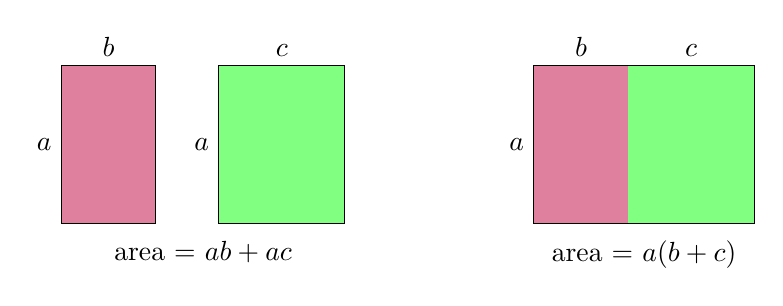
\begin{tikzpicture}[scale=0.4]
	\draw[fill=purple!50] (0,0) rectangle (3,5);
	\draw (0,2.5) node[left]{$a$};
	\draw (1.5,5) node[above]{$b$};
	\draw[fill=green!50] (5,0) rectangle (9,5);
	\draw (5,2.5) node[left]{$a$};
	\draw (7,5) node[above]{$c$};
	\draw (4.5,-0.25) node[below]{area = $ab+ ac$};

	\begin{scope}[shift={(15,0)}]
	\draw[purple!50,fill=purple!50] (0,0) rectangle (3,5);
	\draw (0,2.5) node[left]{$a$};
	\draw (1.5,5) node[above]{$b$};
	\draw[green!50,fill=green!50] (3,0) rectangle (7,5);
	\draw (5,5) node[above]{$c$};
	\draw (0,0) rectangle (7,5);
	\draw (3.5,-0.25) node[below]{area = $a(b+c)$};
	\end{scope}
\end{tikzpicture}
\end{center}
Another way to think about the distributive property is to think of taking the $a$ (in this case) and sprinkling it over the parentheses so that it becomes a part of each of the terms inside.
\begin{center}
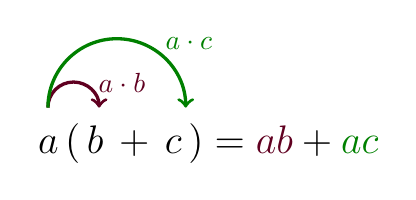
\begin{tikzpicture}
	\draw (0,0) node[right] {\Large$a\,(\,b\,+\,c\,) = {\color{purple!50!black}ab} + {\color{green!50!black}ac}$};
	\draw[purple!50!black, very thick, <-] (0.9, 0.45) arc (0 : 180 : 0.325);
	\draw (0.77, 0.77) node[right] {\color{purple!50!black}$a \cdot b$};
	\draw[green!50!black, very thick, <-] (2, 0.45) arc (0 : 180 : 0.875);
	\draw (1.62, 1.27) node[right] {\color{green!50!black}$a \cdot c$};
\end{tikzpicture}
\end{center}
Both the rectangle-area metaphor and the sprinkling metaphor can be extended to include expressions like \[a(b+c+d) = ab + ac + ad,\] and to expressions with any number of terms inside the parentheses.

%%%%%%%%%%%%%%%%%%%%%%%%%%%%%%%%%%%%%%%%%%%%%%%%%%
\section{Simplified algebraic expressions}
\label{sec:simpalgexpr}

The axioms are a set of tools that we can use to manipulate algebraic objects such that the result is equivalent to the original. That's great\ldots\ but why would we ever need to do that?

Clarity and simplicity are important when it comes to communicating mathematical ideas. The fraction $\frac{16}{24}$ is fine, but the simplified fraction $\frac{2}{3}$ communicates the same information more clearly. For example, it's much easier to visualize a circle with $\frac{2}{3}$ shaded than it is to visualize a circle with $\frac{16}{24}$ shaded.

If a movie starts at 8 o'clock, we would all prefer to see that simple number rather than have to compute $(4+5)\cdot2-10$ o'clock (yes, even algebra teachers feel this way). A simpler form will almost always be easier to understand.

So, as we did with rational numbers and arithmetic expressions, we will define what it means for an algebraic expression to be ``simplified''. Recall from our work in \cref{sec:algexpr} that an \gls{algebraic expression} could be a single term, or the sum of difference of terms. A \gls{term} could be a number, or a variable, or the product/quotient of numbers and variables.

\begin{boxedcriteria}[Criteria for simplified algebraic expressions]
An algebraic expression is considered completely simplified if\ldots
\begin{enumerate}
	\item Numerical expressions have been evaluated
	\item Redundant negative signs have been rewritten
	\item Terms have been arranged in order of decreasing degree, with coefficients written first
	\item It contains no explicit grouping symbols
	\item Different variable terms appear at most once
\end{enumerate}
\end{boxedcriteria}

Several of these criteria are old news. Criteria \#1 just means that we have to simplify numerical expressions using the order of operations: the expression $2 \cdot 3 \cdot x$ is not simplified until we evaluate ``$2 \cdot 3$'' and write ``6'' instead. The equivalent expression $6 \cdot x$ or $6x$ is simplified.

Criteria \#2 is also something we know how to handle. In an expression like $x + \umin6$, where there are two signs in a row, we can simplify using the definition of subtraction: $x + \umin6 = x - 6$.

Criteria \#3 is just a bit of cosmetics. We say that the \gls{degree of a term} is the power to which the variable is raised in a variable term. So, if we have an expression that includes a variable raised to different powers, it's often helpful to see the terms arranged in order from greatest degree to smallest degree. For example, instead of:
\[2x + 3x^4 + 7 - 6x^3 - 18x^2\]
it's often nicer to write:
\[3x^4 - 6x^3 - 18x^2 + 2x + 7\]
Note that when there's a variable with no exponent written, as in the $2x$ here, we think of it has having a ``phantom 1'' in the exponent: $2x = 2x^1$. Also note that the term $7$ has no variable part at all. In this case, we picture a different kind of ``phantom 1'': $7 = 7 \cdot 1 = 7x^0$. If we make these substitutions, we can really see how the terms are arranged by degree:
\[3x^4 - 6x^3 - 18x^2 + 2x^1 + 7x^0\]
Also note that this criteria asks us to write the coefficients first. So, $2x$ is preferred over $x2$. This is, primarily, because it might be tricky to tell the difference between $x2$ and $x^2$. It would be especially confusing in a term has both a coefficient and an exponent: $x^43$ looks a bit too much like $x^{43}$, whereas $3x^4$ is much clearer.

The only criteria left are criteria \#4 and criteria \#5. These are more interesting, and so each gets its own section.

\subsection{Distributive property}

To eliminate grouping symbols, as expressed by criteria \#4, we can rely on the field axioms for help.\footnote{Some special grouping symbols, like the vinculum, can remain in the final expression. Generally, however, we must get rid of grouping symbols that do not double as another operation.} The expression $(x + 2) + 2$ is not simplified, but this can be fixed easily enough using the associative property of addition.
\[(x+2)+2 = x+(2+2) = x+4\]

The expression $3(x + 4)$ is not simplified either, and in this case the distributive property comes to the rescue. Get sprinkling!
\[3(x+4) = 3 \cdot x + 3\cdot 4 = 3x + 12\]

There are subtleties to using the distributive property. Distribution and negative numbers can lead to some easy-to-miss mistakes. We have to be on the lookout, so study the following examples carefully.

\begin{boxedex}
Simplify: (a) $\umin3(2x - 4)$ \quad and \quad (b) $8-5(6x-9)$

\exsoln\ In problem (a) we distribute a negative number. Notice what happens with the signs of the terms in the result.
\[\begin{aligned}
&~ \umin3(2x - 4)&&\\
=&~ \umin3(2x + \umin4)
&& \quad \text{change subtraction to addition of the opposite}\\
=&~ \umin3 \cdot 2x + \umin3 \cdot \umin4
&& \quad \text{distributive property}\\
=&~ (\umin3 \cdot 2)x + \umin3 \cdot \umin4
&& \quad \text{commutative property of multiplication}\\
=&~ \umin6x + 12
&& \quad \text{substitution (in both terms)}\\
\end{aligned}\]
The first thing we did here was to change the subtraction to addition of the opposite. This was helpful because -- look! -- we end up with \textit{positive 12} in the final expression. That might otherwise have been an easy thing to miss.

In problem (b) notice that we have an implied operation that will require us to apply the distributive property. In other words, the first step is \textit{not} to do $8-5$! As with the last problem, we'll start by changing to all-addition.
\[\begin{aligned}
&~ 8-5(6x-9)&&\\
=&~ 8+\umin5(6x + \umin9)
&& \quad \text{change subtraction to addition of the opposite}\\
=&~ 8 + \umin5\cdot6x + \umin5\cdot\umin9
&& \quad \text{distributive property}\\
=&~ 8 + \umin30x + 45
&& \quad \text{substitution}\\
=&~ \umin30x + 8 + 45
&& \quad \text{commutative property of addition}\\
=&~ \umin30x + 53
&& \quad \text{substitution}\\
\end{aligned}\]
Again here, we get a term $\umin5\cdot\umin9 = 45$. Changing to all-addition before distributing is a helpful technique for getting these signs right.
\end{boxedex}

\begin{boxedex}
Simplify: $2x-(x-4)$

\exsoln\ This one is subtle and sneaky! The negative sign is stuck on the parentheses, which means we'll have to ``distribute the negative sign'' or -- more accurately -- we again have an implied operation, hiding in there as a ``phantom one''. This expression is the same as $2x-1(x-4)$.

Observe:
\[\begin{aligned}
&~ 2x-(x-4)&&\\
=&~ 2x-1(x-4)
&& \quad \text{rewrite to expose the ``phantom one''}\\
=&~ 2x + \umin1(x + \umin4)
&& \quad \text{change subtraction to addition of the opposite}\\
=&~ 2x + \umin1x + \umin1\cdot\umin4
&& \quad \text{distributive property}\\
=&~ 1x + 4
&& \quad \text{substitution}\\
=&~ x + 4
&& \quad \text{rewrite to hide the ``phantom one''}\\
\end{aligned}\]
Did you try this problem on your own before reading the solution? Did you get $x-4$? If so, don't be too upset: you're in good company. This is one of the most common mistakes in algebra 1. Always be on the looking when you see the distributive property mixed up with subtraction and negative signs.
\end{boxedex}

\subsection{Combining like terms}

\begin{boxedexplore}[Startup exploration: Expression sort]
Take a moment to sort the following mathematical objects into different groups, creating whatever categories make the most sense to you. After sorting, describe how you made your decisions. What features define each of the groups you have created?

\begin{center}
\begin{tabular}{C{1.5cm}C{1.5cm}C{1.5cm}C{1.5cm}C{1.5cm}C{1.5cm}C{1.5cm}C{0cm}}
17x & 2xy & -4x^2 & 8 & 0.5xy^2 & -y & -15z & \\[2ex]
-3 & 8x^2y & 4y & xy^2 & xyz & 11z & x & \\[2ex]
4xy^2 & -2x^2y & 3xyz & x^2 & -6y & 4x & 3x^2 & \\[2ex]
\end{tabular}
\end{center}
\end{boxedexplore} %% End of startup exploration

One way to sort the terms above is to group \gls{like terms} together. Like terms have the same variable factors raised to the same powers. For example, $17x$ and $4x$ are like terms. Also, $x^2$ and $-4x^2$ are like terms. But, $17x$ and $11z$ are \textit{not} like terms since they have different variable parts. Though it may seem confusing at first, $x$ and $x^2$ are \textit{not} like terms. They both have $x$'s, but those $x$'s are raised to different powers.

\begin{boxedex}[Explaining the startup exploration]
The terms in the startup exploration can be grouped using many different schemes. The categorization below is based on concept of grouping ``like terms'' together.
\begin{itemize}
	\item Terms with no variable: $-3$ and $8$
	\item Terms with $x$ as the variable: $x$, $4x$, and $17x$
	\item Terms with $x^2$ as the variable: $x^2$, $3x^2$, and $-4x^2$
	\item Terms with $y$ as the variable: $-y$, $4y$, and $-6y$
	\item Terms with $z$ as the variable: $-15z$, and $11z$
	\item Terms with $xy$ as the variable: $2xy$
	\item Terms with $x^2y$ as the variable: $-2x^2y$, and $8x^2y$
	\item Terms with $xy^2$ as the variable: $0.5xy^2$, $xy^2$, and $4xy^2$
	\item Terms with $xyz$ as the variable: $xyz$ and $3xyz$
\end{itemize}

\end{boxedex}

Just as 3 goats and 2 goats combine to make 5 goats, so too do $3x$ and $2x$ combine to make $5x$. Similarly, $8x^2 + x^2 = 9x^2$ (in this case, $x^2$ really means $1x^2$: there's a phantom 1 lurking there as the coefficient).

The expression $3xy^2 + 3x^2y + 3x^2y^2$ is simplified, since the variables and their corresponding powers do not match (look closely!).

The process of uniting like terms under a single coefficient is called \gls{combining like terms}.\footnote{Also sometimes called ``collecting'' like terms, or ``gathering'' like terms, and sometimes abbreviated ``CLT''.} This is not technically a property in itself, but a ``shortcut'' for a somewhat longer chain of events:
\[\begin{aligned}
	&~ 3x + 2x\\
=	&~ x(3 + 2)
&& \quad \text{the distributive property, in reverse}\\
=	&~ x(5)
&& \quad \text{substitution}\\
=	&~ 5x
&& \quad \text{commutative property of multiplcation}\\
\end{aligned}\]

At first, it's best to commute the terms and group them up. Then we can add up the coefficients of the like terms. We'll see this approach, and a shortcut, in the examples below.

\begin{boxedex}
Simplify: $3x^2 + 2x - 2 + x^3 + 4x^2 - 3x - 2x^3 + 8$

\exsoln\ To make sure we keep track of the signs, we'll convert to all-addition and then move the terms around to put like terms next to each other.
\[\begin{aligned}
	&~ 3x^2 + 2x - 2 + x^3 + 4x^2 - 3x - 2x^3 + 8\\
=	&~ 3x^2 + 2x + \umin2 + x^3 + 4x^2 + \umin3x + \umin2x^3 + 8
&& \quad \text{definition of subtraction}\\
=	&~ x^3 + \umin2x^3 + 3x^2 + 4x^2 + 2x + \umin3x + \umin2 + 8
&& \quad \text{commutative property of addition}\\
=	&~ \umin1x^3 + 7x^2 + \umin x + 6
&& \quad \text{combine like terms}\\
=	&~ x^3 + 7x^2 - x 6
&& \quad \text{simplify signs}\\
\end{aligned}\]
\end{boxedex}

\begin{boxedex}
Simplify $3x-4y+2-5x+7y-6+8y$

\exsoln\ There is no commutative property of subtraction, remember, so we can rewrite all subtraction into adding the opposite, as in the previous example. A shortcut is to remember that \textit{the sign goes with the term} when you rearrange. Really, this is why we rewrite subtraction in the first place! If we're careful, though, we can avoid the rewriting step.

If we look at the given expression, we see that there are three ``types'' of terms that need combining: terms with $x$, terms with $y$ and constant terms (numbers).

Let's pick a type of term (let's choose ones with $x$) and group them up -- signs and all! In the given expression, we have $3x-5x$, to we have $\umin2x$ in all.

Pick another type of term and repeat as necessary! If we look at the $y$ terms, we have $-4y+7y+8y$ so that's $11y$ in all. Looking at the constant terms, we have $2-6 = \umin4$.

Putting it together, we have $\umin2x + 11y + \umin4$ or (after simplifying signs) $\umin2x + 11y -4$.
\end{boxedex}


% % % % % % % % % % % % % % % % % % % % % % % % % % % % % % % % % % % % % % % % 
\section{Properties of equality (POEs)}
\label{sec:propertiesofequality}

\begin{boxedexplore}[Extended exploration: Mystery numbers]
\addtodoitem{Click here to visit the extended exploration: Mystery Numbers}
\end{boxedexplore}

\begin{boxedexplore}[Startup exploration: Cheese scale]
Bob put a block of edam cheese and three wheels of gouda on one side of a two-pan balance. On the other pan he put seven wheels of gouda. He discovered that the scale was in perfect balance.

\begin{center}
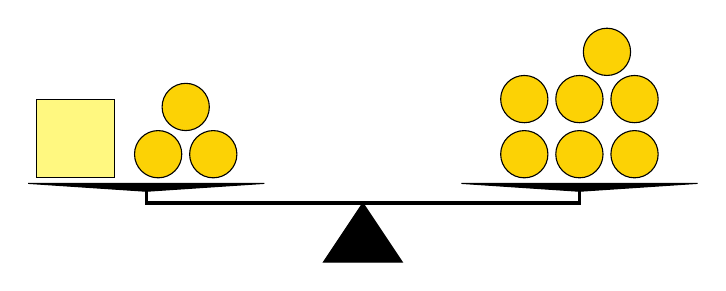
\begin{tikzpicture}
	%%% Left-hand pan, local coordinates (0,0) -- (3,0)
	\begin{scope}
		\draw[fill=yellow!50] (0.1,0) rectangle (1.1,1);
		\draw[fill=yellow!85!red] (1.65,0.3) circle[radius = 0.3];
		\draw[fill=yellow!85!red] (2.35,0.3) circle[radius = 0.3];
		\draw[fill=yellow!85!red] (2,0.9) circle[radius = 0.3];
	\end{scope};
	%%% Right-hand pan, local coordinates (0,0) -- (3,0)
	\begin{scope}[xshift=5.5cm]
		\draw[fill=yellow!85!red] (0.8,0.3) circle[radius = 0.3];
		\draw[fill=yellow!85!red] (1.5,0.3) circle[radius = 0.3];
		\draw[fill=yellow!85!red] (2.2,0.3) circle[radius = 0.3];
		\draw[fill=yellow!85!red] (0.8,1) circle[radius = 0.3];
		\draw[fill=yellow!85!red] (1.5,1) circle[radius = 0.3];
		\draw[fill=yellow!85!red] (2.2,1) circle[radius = 0.3];
		\draw[fill=yellow!85!red] (1.85,1.6) circle[radius = 0.3];
	\end{scope};
	%%% The scale
	\begin{scope}[yshift=-2]
		\draw[fill] (0,0) -- (3,0) -- (1.5,-0.1) -- cycle;
		\draw[very thick] (1.5,0) -- (1.5,-0.25) -- (7,-0.25) -- (7,0);
		\draw[fill] (5.5,0) -- (8.5,0) -- (7,-0.1) -- cycle;
		\draw[fill] (4.25,-0.25) -- (4.75,-1) -- (3.75,-1) -- cycle;
	\end{scope};
\end{tikzpicture}
\end{center}
If all of the wheels of gouda are identical in weight, how many wheels will balance the block of edam?
\end{boxedexplore} %% End of startup exploration

If Bob removes a wheel of gouda from the right-hand pan, it will tip the scales\ldots\ unless he also removes an equivalent amount of gouda from the left-hand pan. In particular, the scale will still be in balance after Bob removes three wheels from each pan of the balance.\footnote{Edam and gouda are traditional Dutch cheeses. Every summer the city of Alkmaar, in the Netherlands, hosts an open-air cheese market. Cheese merchants demonstrate how cheese was bought and sold in medieval times. It operates on Waagplein, which means ``weighing square'' in Dutch, because once the buyer and seller agreed on a price, the huge wheels of cheese were taken to the scales by official ``cheese carriers'', and then weighed very carefully to determine their value. The cheese carriers' guild was established in 1593.}

\begin{center}
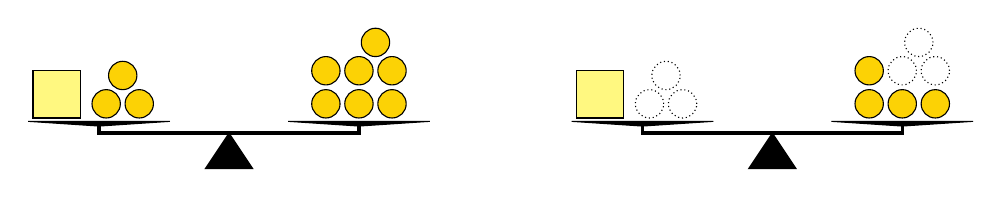
\begin{tikzpicture}[scale=0.6]
	%%% Left-hand pan, local coordinates (0,0) -- (3,0)
	\begin{scope}
		\draw[fill=yellow!50] (0.1,0) rectangle (1.1,1);
		\draw[fill=yellow!85!red] (1.65,0.3) circle[radius = 0.3];
		\draw[fill=yellow!85!red] (2.35,0.3) circle[radius = 0.3];
		\draw[fill=yellow!85!red] (2,0.9) circle[radius = 0.3];
	\end{scope};
	%%% Right-hand pan, local coordinates (0,0) -- (3,0)
	\begin{scope}[xshift=5.5cm]
		\draw[fill=yellow!85!red] (0.8,0.3) circle[radius = 0.3];
		\draw[fill=yellow!85!red] (1.5,0.3) circle[radius = 0.3];
		\draw[fill=yellow!85!red] (2.2,0.3) circle[radius = 0.3];
		\draw[fill=yellow!85!red] (0.8,1) circle[radius = 0.3];
		\draw[fill=yellow!85!red] (1.5,1) circle[radius = 0.3];
		\draw[fill=yellow!85!red] (2.2,1) circle[radius = 0.3];
		\draw[fill=yellow!85!red] (1.85,1.6) circle[radius = 0.3];
	\end{scope};
	%%% The scale
	\begin{scope}[yshift=-2]
		\draw[fill] (0,0) -- (3,0) -- (1.5,-0.1) -- cycle;
		\draw[very thick] (1.5,0) -- (1.5,-0.25) -- (7,-0.25) -- (7,0);
		\draw[fill] (5.5,0) -- (8.5,0) -- (7,-0.1) -- cycle;
		\draw[fill] (4.25,-0.25) -- (4.75,-1) -- (3.75,-1) -- cycle;
	\end{scope};
	%%% implies...
	\draw (10,0) node {\Large$\implies$};
	%%% second drawing...
	\begin{scope}[xshift=11.5cm]
		\begin{scope}
			\draw[fill=yellow!50] (0.1,0) rectangle (1.1,1);
			\draw[fill=white, densely dotted] (1.65,0.3) circle[radius = 0.3];
			\draw[fill=white, densely dotted] (2.35,0.3) circle[radius = 0.3];
			\draw[fill=white, densely dotted] (2,0.9) circle[radius = 0.3];
		\end{scope};
		%%% Right-hand pan, local coordinates (0,0) -- (3,0)
		\begin{scope}[xshift=5.5cm]
			\draw[fill=yellow!85!red] (0.8,0.3) circle[radius = 0.3];
			\draw[fill=yellow!85!red] (1.5,0.3) circle[radius = 0.3];
			\draw[fill=yellow!85!red] (2.2,0.3) circle[radius = 0.3];
			\draw[fill=yellow!85!red] (0.8,1) circle[radius = 0.3];
			\draw[fill=white, densely dotted] (1.5,1) circle[radius = 0.3];
			\draw[fill=white, densely dotted] (2.2,1) circle[radius = 0.3];
			\draw[fill=white, densely dotted] (1.85,1.6) circle[radius = 0.3];
		\end{scope};
		%%% The scale
		\begin{scope}[yshift=-2]
			\draw[fill] (0,0) -- (3,0) -- (1.5,-0.1) -- cycle;
			\draw[very thick] (1.5,0) -- (1.5,-0.25) -- (7,-0.25) -- (7,0);
			\draw[fill] (5.5,0) -- (8.5,0) -- (7,-0.1) -- cycle;
			\draw[fill] (4.25,-0.25) -- (4.75,-1) -- (3.75,-1) -- cycle;
		\end{scope};
	\end{scope}
\end{tikzpicture}
\end{center}

Taking three wheels from each side of the balance is helpful because it means that we will have gotten the block of edam alone on one side. From there it's easy to see that the block weighs the same as four wheels.

The idea of maintaining balance is the heart of the algebra of solving equations.

\begin{boxeddef}[Equation]
An \gls{equation} is a number sentence which states that two algebraic expressions are equal.
\end{boxeddef}

To create an algebraic version of the balance problem, we need a way to represent the weight of the block of edam. In other words, we need a way to write down the weight of the block \textit{before we know what the weight actually is}.

\begin{boxeddef}[Unknown]
An \gls{unknown} is a quantity whose value is not known. We usually represent an unknown using a letter.

Both variables and unknowns are represented by letters though, technically speaking, an unknown is different from a variable. A variable's value can vary or change, whereas an unknown has a fixed value (or set of values) that must be determined.
\end{boxeddef}

Let's use $B$ to stand for the unknown weight of the block, and let's assume that each wheel weighs 1 unit. Then, we can translate our balance problem into algebraic symbols: \[B + 3 = 7.\] If we take three (wheels) from each side of the balance, we have \[B = 4\] which tells us that $B$, the weight of the block, is four units. Our key task here was transforming the first equation into the second equation.

In \cref{sec:equivalence} we used the field axioms to simplify individual algebraic expressions. An equation is a math sentence with an expression on each side of the equal sign. So, we need some rules that will allow us to manipulate two expressions at the same time, but in such a way that their equality remains intact.

\subsection{Maintaining equality}

An equation states that the two pans of a balance (the expressions on either side of the equal sign) are in alignment. If we were to, say, add five to the expression on one side of the equation, then we would tip the scales out of balance\ldots\ unless we also add five to the expression on other side of the equation.

This idea, and others like it, are captured mathematically is a set of rules called the Properties of Equality, or POEs for short.

\begin{boxeddef2col}[Properties of equality: Addition and subtraction]
The \gls{addition property of equality} (APOE) states that for all real numbers $a$, $b$, and $c$ \[\text{if } a = b \text{, then } a + c = b + c\]
\tcblower
The \gls{subtraction property of equality} (SPOE) states that for all real numbers $a$, $b$, and $c$\[\text{if } a = b \text{, then } a - c = b - c\]
\end{boxeddef2col}

Note that since ``subtraction'' is the same as ``addition of the opposite'', SPOE is really just APOE in disguise.

\begin{boxeddef2col}[Properties of equality: Multiplication and division]
The \gls{multiplication property of equality} (MPOE) states that for all real numbers $a$, $b$, and $c$, where $c\neq 0$ \[\text{if } a = b \text{, then } a \cdot c = b \cdot c\]
\tcblower
The \gls{division property of equality} (DPOE) states that for all real numbers $a$, $b$, and $c$, where $c\neq 0$ \[\text{if } a = b \text{, then } \frac{a}{c} = \frac{b}{c}\]
\end{boxeddef2col}

Here again, note that since ``division'' is the same as ``multiplication by the reciprocal'', DPOE is really just MPOE in disguise. Note too that $c$ must not equal 0 when using these rules. Using 0 with DPOE must certainly be avoided, lest we be flummoxed upon division by zero.\footnote{Why must we be cautious about multiplying both sides of an equation by zero? In the end we'll get $0=0$, which is a true statement. What's the problem? Note that multiplication by 0 is \textit{irreversible}. If we multiply by 2 (or any nonzero number) we can reverse or ``undo'' this operation by dividing by 2. But, since division by 0 is not allowed, we cannot undo multiplication by 0. Later, we will see that irreversible operations can lead us to ``fake'' solutions to our equations, so-called \textit{extraneous solutions}.}

Let's use the properties of equality to solve the problem of Bob's cheese balance.

\begin{boxedex}
Bob put a block of edam cheese and three wheels of gouda on one side of a two-pan balance. On the other pan he put seven wheels of gouda. He discovered that the scale was in perfect balance. If all of the wheels of gouda are identical in weight, how many wheels will balance the block of edam?

\exsoln\ Let $B$ represent the weight of the block of edam. Then, the given information suggests the equation $B + 3 = 7$. We want to isolate $B$.
\[\begin{aligned}
B + 3 & = 7\\
B + 3 {\color{red} \,-\,3} & = 7 {\color{red} \,-\,3}
&&\text{\quad SPOE: subtract 3 from both sides of the equation}\\
B & = 4
\end{aligned}\]
\end{boxedex}

Note that in our work above, we started out by defining what variable we would use to represent our unknown. Then, we wrote an equation based on the information given in the problem. Our goal was to get $B$ by itself on one side of the equation, or to \textit{isolate $B$}. Since 3 had been added to $B$, we had to ``undo'' this. So, we subtracted 3 from both sides using SPOE.

\begin{boxeddef}[Inverse operations (a.k.a. opposite operations)]
Operations that will ``undo'' one another. For example, addition and subtraction are inverse operations. Multiplication and division are inverse operations.
\end{boxeddef}

When we solve an equation, we use inverse operations to undo the order of operations. Once we get a hang of the rules, solving equations can become a game. Plus, like the best video games, equation-solving has different levels of challenge so that the game stays interesting even as you get better and better at it.


% % % % % % % % % % % % % % % % % % % % % % % % % % % % % % % % % % % % % % % % 
\section{Level 1 and 2 linear equations}
\label{sec:linearlevels1and2}

\subsection{Level 1 equations}

Level 1 linear equations are the simplest kind to solve because it takes only one step to isolate the variable. The example we saw in the last section was a Level 1 linear equation.

\begin{boxedex}
Consider each of the equations below. What step should we perform to isolate the variable?

\begin{tabular}{C{0.2\linewidth}C{0.2\linewidth}C{0.2\linewidth}C{0.2\linewidth}}
x\div 4 = 21 & w - 9 = 50 & y + 13 = \umin24 & 8 x = 72\\
\end{tabular}

\expsoln\ In the first equation we must multiply both sides of the equation by 4 (MPOE).
\[\begin{aligned}
x \div 4& = 21\\
\frac{x}{4}& = 21
&&\text{\quad definition of division}\\[2ex]
\frac{x}{4} {\color{red} \,\cdot\,4} & = 21 {\color{red} \,\cdot\,4}
&&\text{\quad MPOE: multiply both sides of the equation by 4}\\[2ex]
x & = 84
\end{aligned}\]
In the second equation we should add 9 to both sides (APOE). In the third equation, we should subtract 13 (SPOE). Alternatively, we can think of this as APOE in which we add $\umin13$ to both sides.

In the last example, we should divide both sides of the equation by 8 (DPOE). Or, we can think of this as MPOE in which we multiply both sides by $\frac{1}{8}$.
\end{boxedex}

\subsection{Level 2 equations}

Here's an example of a level 2 equation. How is it different from Level 1? \[3x + 16 = 43\]
Notice that in this equation, two things were done to the unknown $x$. First it was multiplied by 3, and then 16 was added to the result. To isolate the variable, the rule of thumb is to undo whatever was done to the unknown. Usually this means that we will have to undo the order of operations in reverse. Most of the time, we can rely on the ``underpants analogy''.

\begin{boxeddef}[Underpants analogy]
When you get dressed for school in the morning, you put your underpants on \textit{before} you put on your jeans. When you get undressed to go to bed, you do the \textit{opposite} of each step, and you do the steps in the \textit{opposite order}. In other words: you have to take your jeans off first, before you can take your underpants off.\footnote{Try doing it the other way around, we dare you. Later.}
\end{boxeddef}

To undo the order of operations, we have to work upside-down and backwards:
\[\begin{aligned}
3x + 16 & = 43\\
3x + 16 - 16 & = 43 - 16
&&\text{\quad SPOE: subtract 16 from both sides of the equation}\\
3x & = 27
&&\text{\quad Simplify and substitute}\\[1ex]
\frac{3x}{3} & = \frac{27}{3}
&&\text{\quad DPOE: divide both sides of the equation by 3}\\[1ex]
x & = 9
&&\text{\quad Simplify and substitute}\\
\end{aligned}\]
In the end we have isolated $x$, and so this final equation tells us that 9 is a solution to the original equation.

\begin{boxeddef}[Solution and solution set]
A \gls{solution} to an equation is any value that will make the equation true.

Sometimes an equation will have more than one solution. The set of all solutions to an equation are called a \gls{solution set}. To write a solution set, we use set notation and write $\solset{list ~ of ~ solutions}$.
\end{boxeddef}

As we go through the process of solving an equation, each application of a Property of Equality produces an equation that is equivalent to the original.

\begin{boxeddef}[Equivalent equations]
Equations that have the same solution set.
\end{boxeddef}

\subsection{Showing and checking work}

As with problems that involved the order of operations, it is often best to show your work going down the page as we have done in the earlier sections. It is also very helpful to anyone reading your work if you write beside each step the property that you used to justify turning one equation into an equivalent equation.

A note on vocabulary: we \textit{simplify and expression} and we \textit{solve an equation}. Even though the work we show might be very similar, the goal of our steps is quite different.

Having found a solution, it is a great habit to check the solution by substituting it back into the original equation. In the example above, we had the equation $3x+16=43$ and found that this was equivalent to the equation $x=9$. To check our solution, we plug 9 back in for $x$ in the original equation:
\[\begin{aligned}
3x + 16 & = 43
&&\quad\text{original equation}\\
3(9) + 16 & \overset{?}{=} 43
&&\quad\text{substitute in 9 for $x$}\\
27 + 16 & \overset{?}{=} 43
&&\quad\text{carry out the order of operations}\\
43 & \overset{\checkmark}{=} 43
&&\quad\text{Check!}
\end{aligned}\]
When we substitute in 9, we put little question marks over out equal sign, since we are checking the solution -- we're not sure whether the two expressions are equal yet! In the end, when we discover that the left-hand side is equal to the right-hand side, we replace our question with a check mark of confirmation!

The key here is to realize that, ultimately, the process we use to solve an equation yields \textit{candidates} for the value of the unknown. We are not guaranteed that all of these candidates actually satisfy the original equation, until we check them to know for sure.\footnote{There will come a time when we will do everything correctly, and still some of our solution-candidates will have to be rejected! Get in the habit of checking solutions now!}

Once we have verified that our solution satisfies the original equation, we should write our answer in set notation. The equation $x=5$ isn't our solution, but an equivalent equation -- in fact, it's the simplest equation that has the same solution as the original!

In other words, the equation solving process creates simpler and simpler equations that all have the same solution. Eventually, we get to the an equation that shows the solution clearly. We use set notation to record our solution because it is a notation that suggests the solution works for all of the intermediate equations.

Plus, solution set notation works nicely with all types of equations. Soon we will have equations with multiple solutions (even infinitely many!) and the $x=$ notation starts to be become quite awkward.

So, in our ongoing example, we write $\solset{5}$. Yes, a mathematical ``set'' may contain just a single element!\footnote{This is another situation in which we find a conflict between everyday language and the language of mathematics. Lots of words have a special meaning when used in a mathematical context: similar, odd, mean, product\ldots\ What other examples can you think of?} The alternative to using solution set notation is to write the sentence ``The solution to the equation is 5.''


% % % % % % % % % % % % % % % % % % % % % % % % % % % % % % % % % % % % % % % % 
\section{Level 3 linear equations: Multiple steps}
\label{sec:linearlevel3}

Level 1 equations are called, naturally enough, \textit{one-step equations}, and Level 2 equations are called -- you guessed it! -- two-step equations. In Level 3, we increase complexity by combining the tasks of expression-simplifying and equation-solving.

\begin{boxedexplore}[Extended exploration: Evil mystery numbers]
\addtodoitem{Click here to visit the extended exploration: Evil Mystery Numbers}
\end{boxedexplore}

\begin{boxedexplore}[Startup exploration: Linear level 3]
Determine the value $x$, given the equation \[2x + 7 - 5x + 12 = 15.\]
\end{boxedexplore} %% End of startup exploration

Here we find an equation that must be simplified using the field axioms and related tools. Let's start out by trying to simplify the left-hand side.
\[\begin{aligned}
2x + 7 - 5x + 12 & = 15\\
2x + 7 + \umin5x + 12 & = 15
&&\text{\quad rewrite as addition, by def'n of subtraction}\\
2x + \umin5x + 7 + 12 & = 15
&&\text{\quad commutative property of addition}\\
\umin3x + 19 & = 15
&&\text{\quad combine like terms -- this is now a Level 2 equation!}\\
\umin3x + 19 - 19 & = 15 - 19
&&\text{\quad SPOE}\\
\umin3x & = \umin4
&&\text{}\\[1ex]
\frac{\umin3x}{\umin3} & = \frac{\umin4}{\umin3}
&&\text{\quad DPOE}\\[1ex]
x & = \frac{4}{3}
&&\text{\quad Simplify}\\[1ex]
\end{aligned}\]

Notice that after a few lines, we had turned the Level 3 equation into a Level 2 equation. We know how to solve those! So, our goal will be to try to turn Level 3 equations into a Level 1 or Level 2 equations. But, since there are more steps in the process, there's more chance we can make a mistake. So, it's a good habit to remember to check our answer at the end.

We can check our answer for the last problem by substituting our solution back into the original equation and simplifying using the order of operations.
\[\begin{aligned}
2x + 7 - 5x + 12 & = 15
&& \text{\quad original equation}\\
2\left(\frac{4}{3}\right) + 7 - 5\left(\frac{4}{3}\right) + 12 & \overset{?}{=} 15
&& \text{\quad substitute in our solution $x = \tfrac{4}{3}$}\\[1ex]
2\left(\frac{4}{3}\right) + 7 + \umin5\left(\frac{4}{3}\right) + 12 & \overset{?}{=} 15
&& \text{\quad rewrite as addition, by def'n of subtraction}\\[1ex]
\frac{8}{3} + 7 + \frac{\umin20}{3} + 12 & \overset{?}{=} 15
&& \text{\quad multiply fractions}\\[1ex]
\frac{8}{3} + \frac{21}{3} + \frac{\umin20}{3} + \frac{36}{3} & \overset{?}{=} 15
&& \text{\quad rewrite left-hand side with common denominator}\\[1ex]
\frac{45}{3} & \overset{?}{=} 15
&& \text{\quad add fractions}\\[1ex]
15 & \overset{\checkmark}{=} 15
&& \text{\quad boom!}
\end{aligned}\]
Writing our solution as a solution set, we have $\solset{15}$.

\begin{boxedex}
\label{ex:dist}
Determine the value of $w$, given the equation \[7w + 2(\umin3w + 1) = 12.\]

\exsoln\ Our goal is to try and simplify the left-hand side so that it looks like a Level 1 or Level 2 equation.
\[\begin{aligned}
7w + 2(\umin3w + 1) &= 12\\
7w + \umin6w + 2 &= 12
&&\text{\quad distributive property}\\
1w + 2 & = 12
&&\text{\quad combine like terms -- that's a Level 1 equation!}\\
w + 2 - 2 & = 12 - 2
&&\text{\quad SPOE}\\
w & = 10
\end{aligned}\]
Let's check our solution:
\[\begin{aligned}
7w + 2(\umin3w + 1) &= 12
&& \text{\quad original equation}\\
7(10) + 2(\umin3(10) + 1) &\overset{?}{=} 12
&& \text{\quad substitute in our solution $w = 10$}\\
70 + 2(\umin30 + 1) &\overset{?}{=} 12
&& \text{\quad carry out the order of operations on the left-hand side}\\
70 + 2(\umin29) &\overset{?}{=} 12\\
70 + \umin58 &\overset{?}{=} 12\\
12 &\overset{\checkmark}{=} 12\\
\end{aligned}\]
\end{boxedex}

We're going to look at one more example, and discuss two alternative ways to approach it.

\begin{boxedex}
\label{ex:nodist}
Determine the value of $g$, given the equation \[\umin4(2g - 7) = 36.\]

\exsoln\ Approach \#1. Those parentheses are just asking to be simplified using the distributive property. Be mindful of the signs, though!
\[\begin{aligned}
\umin4(2g - 7) &= 36\\
\umin8g + 28 &= 36
&&\text{\quad distributive property -- that's a Level 2 equation!}\\
\umin8g + 28 - 28 &= 36 - 28
&&\text{\quad SPOE}\\
\umin8g &= 8\\[1ex]
\frac{\umin8g}{\umin8} &= \frac{8}{\umin8}
&&\text{\quad DPOE}\\
g &= \umin1
\end{aligned}\]

Approach \#2. Let's solve the same equation again. This time, notice that we can divide both sides by $\umin4$ as the first step, which eliminates the need for the distributive property.
\[\begin{aligned}
\umin4(2g - 7) &= 36\\[1ex]
\frac{\umin4(2g-7)}{\umin4} &= \frac{36}{\umin4}
&&\text{\quad DPOE}\\
2g-7 &= \umin9
&&\text{\quad simplify -- that's a Level 2 equation!}\\
2g-7+7 &= \umin9+7
&&\text{\quad APOE}\\
2g &= \umin2
&&\text{\quad}\\[1ex]
\frac{2g}{2} &= \frac{\umin2}{2}
&&\text{\quad DPOE}\\
g &= \umin1
\end{aligned}\]

\end{boxedex}

The two different approaches taken in the previous example are not always available. Compare the solutions to \cref{ex:dist,ex:nodist}. Can we avoid the distributive property in \cref{ex:dist}? Why or why not?


\subsection{More on checking work}

Every step we take in solving an equation generates an equivalent equation that has the same solution set. If we make a mistake, we accidentally create an equation with a different solution set. Knowing this can help us check our answers on the more complex equations (ones that have more steps).

\begin{boxedex}
Solve for $x$, given the equation $2x-3(4x-1)=-53$.

Let's say we mess up the signs when carrying out the distributive property -- a very common mistake.
\[\begin{aligned}
2x - 3(4x-1) &= \umin53
&& \text{\quad Line 1.}
\\
2x - 12x - 3 &= \umin53
&& \text{\quad Line 2. That's a mistake!}
\\
\umin10x - 3 &= \umin53
&& \text{\quad Line 3.}
\\
\umin10x &= \umin50
&& \text{\quad Line 4.}
\\
x &= 5
&& \text{\quad Line 5.}
\end{aligned}\]

Now, we go back to check our work by substituting the solution into the original equation. The answer doesn't work in line 1, so we know it is not the correct solution. \[2(5) - 3\bigl(4(5)-4\bigr) = \umin53 \implies \umin38 \neq \umin53 \text{\quad(something went wrong!)}\]
But, our answer \textit{does} work in line 2 (and also lines 3,4, and 5).
\[2(5) - 12(5) - 3 = \umin53 \implies \umin53 = \umin53 \text{\quad(that works!)}\]
This is the clue helps us pinpoint the location of the mistake. It tells us the mistake must have happened when transforming line 1 into line 2.

If, on a different problem, we find that our solution doesn't work for steps 1, 2, or 3, but \textit{does work} in step 4, then it means that our mistake must have happened when transforming step 3 into step 4!
\end{boxedex} 

% % % % % % % % % % % % % % % % % % % % % % % % % % % % % % % % % % % % % % % % 
\section{Level 4 linear equations: Variables on both sides}
\label{sec:linearlevel4}

In Level 4, we add a wrinkle, which can lead to some very unusual results.

\begin{boxedexplore}[Extended exploration: Super evil mystery numbers]
\addtodoitem{Click here to visit the extended exploration: Super Evil Mystery Numbers}
\end{boxedexplore}

\begin{boxedexplore}[Startup exploration: Linear level 4]
Determine the value of $x$ given the equation \[13x-5x-5=x+7+x.\]
\end{boxedexplore} %% End of startup exploration

The goal is the same: to isolate the variable on one side of the equal sign. We begin by simplifying each side.
\[\begin{aligned}
13x-5x-5 &= x+7+x\\
8x-5 &= 2x+7
&&\text{\quad combine like terms on both sides}\\
8x-5 - 2x &= 2x+7 - 2x
&&\text{\quad SPOE: subtract $2x$ from both sides -- clever!}\\
6x-5 &= 7
&&\text{\quad combine like terms again -- that's a Level 2 equation!}\\
6x &= 12
&&\text{\quad APOE: add 5 to both sides}\\
x &= 2
&&\text{\quad DPOE: divide both sides by 6}
\end{aligned}\]
In this example, we subtracted $2x$ from both sides of the equation. This might seem like a tricky move, but it's a completely legal application of SPOE. We are allowed to do the same thing to both sides of the balanced equation, even if that means subtracting an unknown amount from both sides.\footnote{Of course, you have to subtract the same unknown amount from both sides. It's no fair to subtract $x$ from one side of an equation and $y$ from the other side. This will put the equation out of balance unless we know that these two unknown amounts are equal\ldots\ that is, unless we know that $x=y$. Caution: can you think of a situation in which it might be dangerous to apply a POE using an unknown? Think about what might happen if we use DPOE to divide both sides by an unknown value $x$.}

Let's see what happens if we isolate the unknown on \textit{the other side of the equal sign}. (It had better give us the same answer!)
\[\begin{aligned}
13x-5x-5 &= x+7+x
&&\text{\quad same equation as before}\\
8x-5 &= 2x+7
&&\text{\quad combine like terms on both sides, as before}\\
8x-5 - 8x &= 2x+7 - 8x
&&\text{\quad SPOE: subtract $8x$ from both sides}\\
\umin5 &= \umin6x + 7
&&\text{\quad combine like terms}\\
\umin12 &= \umin6x
&&\text{\quad SPOE: subtract 7 from both sides}\\
2 &= x
&&\text{\quad DPOE: divide both sides by $\umin6$}
\end{aligned}\]

So, it doesn't matter which side we choose to eliminate the unknown. As long as we apply APOE or SPOE correctly, the solution will be the same. One strategy is to choose the side that will result in a \textit{positive coefficient} for the variable. This isn't required, but it helps avoid the chances of losing a negative sign along the way (maybe that's happened to you).\footnote{Napoleon ordered the creation of the first modern lost-and-found office in Paris in 1805, although lost-property systems have existed in Japan since the early 700s.}

Plus, if you don't like the side of the equation that the unknown is on, you can always rewrite the equation. For example if you have the equation $3=4+x$ and you really want the $x$ on the left-hand side, you can just rewrite the equation as $4+x=3$. Those are equivalent equations!\footnote{Even these obvious properties have been given names. For example, this is a fact about equations: if $a=b$, then $b=a$. To describe this, we say that equality is \textit{symmetric}. An even more obvious statement is that $a=a$ (we say that equality is \textit{reflexive}). A third property is a little more interesting: if $a=b$ and $b=c$, then $a=c$ (we say that equality is \textit{transitive}). }

\begin{boxedex}
Determine the value of $x$ given the equation \[3(x-2)+3x=4x-6.\]

\exsoln\ Let's jump right in and start simplifying the left-hand side.
\[\begin{aligned}
3(x-2)+3x &= 4x-6\\
3x-6+3x &= 4x-6
&&\text{\quad distributive property}\\
6x-6 &= 4x-6
&&\text{\quad combine like terms}\\
2x-6 &= -6
&&\text{\quad SPOE: subtract $4x$ from both sides}\\
2x &= 0
&&\text{\quad APOE: add 6 to both sides}\\
x &= 0
&&\text{\quad DPOE: divide both sides} by 2\\
\end{aligned}\]

Yes, we can get 0 as the solution to an equation. We can always check to be sure:
\[\begin{aligned}
3(x-2)+3x &= 4x-6
&& \text{\quad original equation}\\
3(0-2)+3(0) &\overset{?}{=} 4(0)-6
&& \text{\quad substitute in our solution $x = 0$}\\
3(\umin2)+0 &\overset{?}{=} \umin6
&& \text{\quad simplify}\\
\umin6 &\overset{\checkmark}{=} \umin6\\
\end{aligned}\]
\end{boxedex}

\subsection{Special cases}

There are some things to be careful about with when it comes to solving Level 4 linear equations. Here is an example of something strange that can happen when we have unknowns on both sides of the equal sign.

\begin{boxedex}
Determine the value of $x$ given the equation \[12x + 36 = 2(6x-10).\]

\exsoln\ We proceed as we have done in earlier problems:
\[\begin{aligned}
12x + 36 &= 2(6x-10)\\
12x + 36 &= 12x-20
&&\text{\quad distributive property}\\
12x+36-12x &= 12x-20-12x
&&\text{\quad SPOE: subtract $12x$ from both sides}\\
36 &= \umin20
&&\text{\quad Huh?}\\
\end{aligned}\]

In this case the variable term disappears completely from both sides of the equation. And then, what is left is obviously \textit{not equal}. In a sense, the original ``equation'' is not an equation at all. The two given expressions are not equal, and never will be.

This means that there is no value of $x$ what will ever work to make the equation true. We say that this equation \textit{has no solution}.
\end{boxedex}

As unsatisfying as it might sound, it is possible to have an equation that does not have a solution.\footnote{Equations without solutions are very important in the history of mathematics. The French mathematician Pierre de Fermat made a conjecture in 1637 stating that a certain equation had no integer solutions. His claim, which came to be known as Fermat's Last Theorem, wasn't officially proven to be correct for more than 350 years. British mathematician Andrew Wiles published the first complete proof of Fermat's Last Theorem in 1995. The theorem states that the equation $a^n + b^n = c^n$ has no integer solutions for $a$, $b$, and $c$ when the exponent $n$ is a natural number greater than 2.}

How do you write down the solution to a problem that has no solution? This is not quite as philosophical as it sounds. We can, of course, write the words ``no solution''. Or, we could write a solution set that contains no numbers, $\solset{~}$.

Or, there is a third option. You may or may not be surprised to learn that mathematicians have invented a symbol for just such an occasion. We use the mathematical symbol \emptyset, called the ``empty set'' or ``null set'', as a way to show that that our solution set is empty.\footnote{The symbol \O, which was introduced by French mathematician Andr\'e Weil in 1939, is a letter in the Norwegian alphabet.} We write $\mathcal{S} = \emptyset$ to mean ``the solution set is empty''.

Notice that we don't write the curly braces around the empty set. In other words, we write $\mathcal{S}=\emptyset$ and not $\solset{\emptyset}$. The former says ``$S$ is the empty set'', which is what we mean when we have an equation with no solutions. The latter says ``$S$ is the set which contains the empty set'' which -- believe it or not -- is not the same thing.\footnote{The empty set is not the same as zero, and it is not the same as nothing. It is a set with nothing inside it, like an empty bag. So, writing $\mathcal{S} = \emptyset$ is stating that the solution set is like an empty bag. Extending this metaphor, $\{\emptyset\}$ is a bag with an empty bag in it and, therefore, a set which contains the empty set is not empty. Om.}

For the record, the empty set is not the same as zero. So, an equation can have the solution set $\solset{0}$, like example 5.6. This is different from an equation having the solution set $\solset{~}$, like example 5.7.

If you look back at the reason why the last example has no solution, you may be wondering about whether there is another possibility. Study the following example.

\begin{boxedex}
Determine the value of $x$ given the equation \[5x-3(x+2)=2x-6.\]

\exsoln\ Let's go for it:
\[\begin{aligned}
5x-3(x+2) &= 2x-6\\
5x-3x-6 &= 2x-6
&&\text{\quad distributive property, watch the signs}\\
2x-6 &= 2x-6
&&\text{\quad combine like terms -- something is fishy already.}\\
2x-6-2x &= 2x-6-2x
&&\text{\quad SPOE: subtract $2x$ from both sides}\\
-6 &= -6
&&\text{\quad But, of course.}\\
\end{aligned}\]

In this case the variable term disappears again, and the leftovers are \textit{obviously equal}. This is the opposite of what happened earlier. If that example had no solutions, this one has all of them. We can replace $x$ with literally any real number and the equation will be true. That means that we have a solution set that contains every real number there is.

We say that this equation's solutions are \textit{all real numbers}.
\end{boxedex}

In this example, our solution set is the set of real numbers. We can write this out in words, ``all real numbers'', or use the shorthand symbol that stands for the real numbers and write, $\mathcal{S} = \R$. Notice no curly braces are used here either.

\subsubsection{Checking answers in special cases}

In the case that we find ``all real numbers'' as as the solution to an equation, we know that every number is going to work. So to check, we might pick a couple of different numbers (easy ones, like 0 and 1) and substitute those into the original equation. Any number that you choose should satisfy the equation.

If we find that an equation has ``no solutions'', then any number we use to check will fail to satisfy the equation. Not very informative. In this case, it may be best just to check back over our work to make sure that we did each of the steps correctly.

%%%%%%%%%%%%%%%%%%%%%%%%%%%%%%%%%%%%%%%%%%%%%%%%%%
\section{Level 5 linear equations: Absolute value}
\label{sec:linearlevel5}

Over the last few sections we have added complexity to the equation-solving picture. We have learned properties that can be used to ``undo'' whatever has been ``done'' to the variable. Sometimes this has led to situations where the equation has no solutions, or infinitely many solutions. We turn now to equations that involve the absolute value of an unknown.\footnote{We're discussing absolute value equations here in the chapter on linear equations, though we put ``linear'' in quotes. Absolute value equations of the kind that we're discussing here are linear-like enough that they fit here. Other types of absolute value equations are possible, though we won't get into the full range of variations in this course.}

\begin{boxedexplore}[Extended exploration: Dreadful mystery numbers]
\addtodoitem{Click here to visit the extended exploration: Dreadful Mystery Numbers}
\end{boxedexplore}

\begin{boxedexplore}[Startup exploration: Linear level 5]
Recall the definition of absolute value. Determine the value of $x$ given the equation \[\abs{x} = 6.\]
\end{boxedexplore} %% End of startup exploration

Recall that the absolute value of a number is that number's distance away from zero on the number line. Distances are always positive: $\umin6$ is 6 units away from 0, and so $\abs{\umin6}=6$. Of course, $\abs{6} = 6$ as well. So, the equation above has two solutions $x = 6 \OR \umin6$.\footnote{Note, we mean \textit{or} and not \textit{and}. Both 6 and $\umin6$ are solutions to the equation, but we must write $x=6 \OR \umin6$, since $x$ can have only take on one value at a time.} In solution set notation, we write $\solset{6, \umin6}$.

The presence of the absolute value gives us the possibility of having two solutions, since whatever is inside the absolute value bars could be either the positive or the negative version of the value.

Here's an extension to the idea. Determine the value of $x$ given the equation \[\abs{2x} = 16\]
This is telling us that the number ``$2x$'' is 16 units away from zero on the number line. In other words \[2x = 16 \OR \umin16.\]
This is really two equations written at once: $2x = 16$ and $2x = \umin16$. We can apply DPOE and divide everything by 2, which will isolate $x$. That is, we have \[x = 8 \OR \umin8.\]

The following two examples carry this idea a bit further.

\begin{boxedex}
Determine the value of $x$ given the equation \[\abs{\umin3x+9} = 12.\]

\exsoln\ The stuff inside the absolute value bars can equal 12 or $\umin12$. So, this means, we have two equations:
\[\begin{aligned}
\umin3x + 9 &= 12 	&\OR 	&&\umin3x + 9 &= \umin12\\
\umin3x  &= 3 		&	 	&&-3x &= \umin21
&&\text{\quad SPOE: subtract 9 throughout}\\
x &= \umin1 		&	 	&&x &= 7
&&\text{\quad DPOE: divide by $-3$ throughout}\\
\end{aligned}\]
This equation has solutions $\solset{\umin1, 7}$.
\end{boxedex}

Note that the steps we took for solving were the same for both equations (in this case, first we used SPOE, and then DPOE). So, we can streamline our work a bit, as shown in the next example.

The next example also has things going on outside of the absolute value symbols. For these types of problems, we want to isolate the absolute value expression first (using the properties of equality), then separate into two equations (if necessary).\footnote{In case you are wondering, we won't get into equations that include multiple abvolute value expressions\ldots\ although you might enjoy exploring an equation of this kind, just for fun. For example, what values of $x$ satisfy this equation? $\abs{x+2}=2\abs{x}-1$}

\begin{boxedex}
Determine the value of $x$ given the equation: $3\abs{\umin4x+4} = 48$.

\exsoln\ 
\[\begin{aligned}
3\abs{\umin4x+4} &= 48\\
\abs{\umin4x+4} &= 16
&&\text{\quad DPOE, to isolate the absolute value expression}\\
\umin4x+4 &= 16 \OR \umin16
&&\text{\quad definition of absolute value}\\
\umin4x &= 12 \OR \umin20
&&\text{\quad SPOE: subtract 4 throughout}\\
x &= \umin3 \OR 5
&&\text{\quad DPOE: divide by $\umin4$ throughout}
\end{aligned}\]
So, this equation has solutions $\solset{\umin3, 5}$.
\end{boxedex}

\subsection{Special considerations}

A few sneaky things can pop up when it comes to absolute value equations. Recall that the only number that has absolute value zero is zero itself: $\abs{0} = 0$. So, not all absolute value equations have \textit{two} solutions. Consider
\[\abs{3x + 51} = 0.\]
We can't split this into two different equations. All we have is
\[3x + 51 = 0,\]
and that's a Level 2 linear equation with just a single solution, $\solset{\umin17}$. To demonstrate another tricky aspect, consider the equation \[\abs{4x} + 16 = 5.\]
No problem! We begin by subtracting 16 from both sides:
\[\abs{4x} = \umin11\]
But, the absolute value of a number can never be negative. So, this equation has no solution. In other words, we have $\mathcal{S} = \emptyset$.

Don't be too quick with the ``no solutions'' talk, though. If we encounter the equation \[\umin3\abs{x + 2} = \umin12,\] we may see the $\umin12$ and assume there is no solution. But recall that we must isolate the absolute value expression first. To do that we will divide both sides by $\umin3$ and then we will have \[\abs{x+2} = 4,\] an equivalent equation that surely has a solution (two solutions, in fact). So, don't jump to conclusions!

\begin{boxedwarning}
Some folks like to use the notation ``plus/minus'' in situations that involve absolute value. For example, writing ``$\pm6$'' with the little stacked-up plus and minus signs to stand for ``$6 \OR \umin6$''. We recommend avoiding $\pm$ notation when solving equations.

Here's why. See if you can spot the error in the following work.
\[\begin{aligned}
\abs{x - 5} &= 12\\
x-5 &= \pm12\\
x &= \pm17
&& \text{\quad APOE: add 5 to both sides}\\
\end{aligned}\]
And so, $\solset{17, \umin17}$. This work looks reasonable, but let's check the two solutions.
\[\abs{17 - 5} \overset{?}{=} 12 \implies \abs{12} \overset{?}{=} 12 \implies 12 \overset{\checkmark}{=} 12\]
\[\abs{\umin17 - 5} \overset{?}{=} 12 \implies \abs{\umin22} \overset{?}{=} 12 \implies 22 \neq 12\]
So, using the $\pm$ notation has led us to get one correct solution and one incorrect solution for the equation! This is why we recommend writing out the word ``or'' explicitly, or breaking into two separate equations.

(By the way, the correct solution is $\solset{17, \umin7}$. Try working out the problem again using a more reliable technique. Can you see exactly where the work using $\pm$ went astray?)
\end{boxedwarning}

%%%%%%%%%%%%%%%%%%%%%%%%%%%%%%%%%%%%%%%%%%%%%%%%%%
\section{Applications of equation solving}
\label{sec:eqsolveapplications}

Now that we know how to handle different types of equations, let's explore a few applications. First, we'll discuss writing (and then solving) equations based on problem situations. Then, we'll see how to apply the properties of equality to manipulate formulas from science and other disciplines. We'll close this chapter with an extension section about explaining some fundamental ideas using the field axioms.

\subsection{Writing equations to solve word problems}

There are lots of ways to approach problems like this: educated guessing-and-checking, wishful thinking, making an organized list, and so on. One way is to model the situation with (and then solve) an equation. Converting a word problem into an equation is an important skill for your mathematical toolbox.

\begin{boxedexplore}[Extended exploration: Mixed bag o' problems]
\addtodoitem{Click here to visit the extended exploration: Mixed Bag 'O Problems}
\end{boxedexplore}

\begin{boxedexplore}[Startup exploration: Trick or treat]
On Halloween night, Hildegaard and Ingvar (Bob and Yeardleigh's parents) had 200 candies in their trick-or-treat bowl. They gave 5 candies to each kid who came to their door, and at the end of the night they had 10 candies left. How many kids came trick-or-treating?
\end{boxedexplore}

The key in word problems like this is first to identify the unknown in the problem. We choose a variable to stand in for the unknown, and write an equation based on the other information given in the problem.

In our example, the unknown is ``how many kids came trick-or-treating'', so let's use $k$ to represent the number of kids. Hildegaard and Ingvar gave 5 candies to every kid, so they gave away $5k$ candies. They started with 200 and gave away $5k$. Giving away suggests subtraction, so they were left with $200-5k$ candies at the end of the night. The problem tells us that they had 10 candies let over, so:
\[200-5k = 10.\]
That's a Level 2 equation! We'll leave it for you to solve and put the solution in the footnote.\footnote{Solving this equation using the POEs leads to the result $k=38$. So, the answer to the question is that 38 kids came trick-or-treating at the Krumbli house on Halloween night.}

Here's a second example. ``Consecutive integer problems'' are a clever type of mystery number problem that might at first appear impossible to solve. There doesn't seem to be enough information! For example: The sum of three consecutive integers is 39. What are the numbers?

What does it mean to have three consecutive integers? Consecutive means ``in an unbroken sequence'', so three consecutive integers are three integers in a row, such as $4, 5, 6$.

Let $N$ represent the smallest of the three consecutive integers. Then, the next integer is $N+1$, and the integer after that is $N+2$. The problem says their sum is 39. So we have
\[\begin{aligned}
N + (N+1) + (N+2) &=  39\\
3N + 3 &= 39
&& \text{\quad combine like terms}\\
3N &= 36
&& \text{\quad SPOE}\\
N &= 12
&& \text{\quad DPOE}\\
\end{aligned}\]
At this point, many students would be tempted to draw a box around their answer and call it a day. After all, we solved the equation, right? But, look back at the question: it asks us to find the \textit{numbers}, plural. Our answer to the question should list all three of the numbers!

What did we actually compute when we solved the equation? We chose $N$ to represent the smallest of the three consecutive integers, and that's 12. So, the full answer is that the three integers are 12, 13, and 14. (A quick check shows that these three do, in fact, add up to 39.)

The moral of the story here is always to check that we are answering the question that has been asked. This step is a helpful way to avoid giving an irrelevant or incomplete solution.

Finally, when it comes to stating the solution to a word problem, we don't usually use set notation. A handy rule of thumb is to think about how we'd say the answer out loud to someone. When we solve an equation with no context, we'd probably say ``The solution is 4.'' Set notation is appropriate, since the answer is just a number, $\solset{4}$.

On the other hand, if we were answering a word problem that asked how many pounds of cream cheese Bob ate, we'd say ``Bob ate 4 pounds of cream cheese.'' When the context of the problem implies a unit on the answer (pounds, dollars, goats, miles per hour), we write the answer and the unit rather than use solution set notation: 4 pounds of cream cheese.

%%%%%%%%%%%%%%%%%%%%%%%%%%%%%%%%%%%%%%%%%%%%%%%%%%
\subsection{Transforming formulas}
\label{sec:transformingformulas}

In all of the examples in this chapter so far, we have solved equations and found the value of an unknown. In this section, we'll discuss a different use the field axioms and the properties of equality.

In the past, you may have learned a formula for the area of a triangle. If we have a triangle with base of length $b$ and height $h$, then its area $A$ has a tidy little formula.
\begin{center}
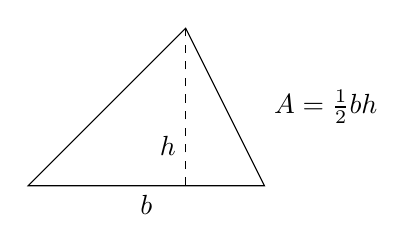
\begin{tikzpicture}[scale=0.5]
	\draw (0,0) -- (6,0) -- (4,4) -- cycle;
	\draw[dashed] (4,0) -- (4,4);
	\draw (4,1) node[left]{$h$};
	\draw (3,0) node[below]{$b$};
	\draw (6,2) node[right]{$A = \frac{1}{2}bh$};
\end{tikzpicture}
\end{center}
If we know the base and height of a specific triangle, we can find its area.
\begin{center}
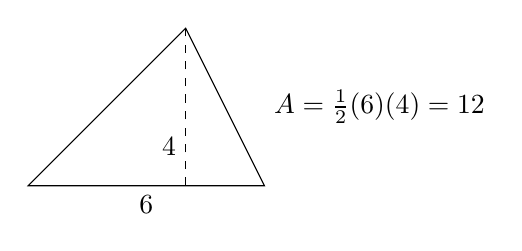
\begin{tikzpicture}[scale=0.5]
	\draw (0,0) -- (6,0) -- (4,4) -- cycle;
	\draw[dashed] (4,0) -- (4,4);
	\draw (4,1) node[left]{$4$};
	\draw (3,0) node[below]{$6$};
	\draw (6,2) node[right]{$A = \frac{1}{2}(6)(4) = 12$};
\end{tikzpicture}
\end{center}
But what if we are given the area and the base length: Could we work backwards to find the height? Could we ``transform'' the area formula so that it computes $h$ instead of $A$?

Transforming a formula means to isolate a specific variable, even though the other side of the equal sign might not simplify down to a single number. The only difference between this and what we have been doing before now is that the equations may have multiple variables (and not unknowns).

\begin{boxedex}
Transform the triangle area formula, $A = \frac{1}{2}bh$, to isolate $h$.

\exsoln\ We'll start with the given formula, and then apply the properties of equality to get $h$ by itself on one side of the equal sign.
\[\begin{aligned}
A &= \frac{1}{2}bh \\[1ex]
2 \cdot A &= 2 \cdot \frac{1}{2} bh
&& \quad\text{MPOE, to eliminate the fraction}\\[1ex]
2A &= bh
&& \quad\text{simplify on the righthand side}\\[1ex]
\frac{2 A}{b} &= \frac{bh}{b}
&& \quad\text{DPOE, to isolate $h$}\\[1ex]
\frac{2 A}{b} &= h
&& \quad\text{simplify on the righthand side: mission accomplished!}\\[1ex]
\end{aligned}\]
So, our transformed formula expresses the height of a triangle in terms of its area and the length of a base: \[h = \frac{2A}{b}\]
\end{boxedex}

This is a skill used in science (especially physics) and higher levels of mathematics. Generally, we have to study the equation we're given and find the variable we are trying to isolate. Then, think about what has been done to that variable which must be undone. We undo these using the POEs.

\addtodoitem{Remember: Since we moved transforming formulas before the linear equations formulae, we should add a bit about transforming standard from later.}

Even though our answers won't be just a number, they should be simplified as much as possible, for instance we must avoid fractions-in-fractions. Parentheses, too, can lead to tricky situations. It often pays to formulate a plan before rushing to work.

\begin{boxedex}
$P = 2( w + d )$ for $w$

\exsoln\ Sometimes we have to distribute, other times it is easier to avoid it all together. Compare the two options below.

Option 1: Avoiding the distributive property
\[\begin{aligned}
P &= 2(w + d)\\
\tfrac{P}{2} &= w - d
&&\quad\text{DPOE}\\
\tfrac{P}{2} - d &= w
&&\quad\text{SPOE}\\
\end{aligned}\]

Option 2: Distributive property first
\[\begin{aligned}
P &= 2(w + d)\\
P &= 2w + 2d
&&\quad\text{distributive property}\\
P - 2d &= 2w
&&\quad\text{SPOE}\\
\tfrac{P - 2d}{2}&= w
&&\quad\text{DPOE}\\
\tfrac{P}{2} - \tfrac{2d}{2}&= w
&&\quad\text{undo fraction subtraction}\\
\tfrac{P}{2} - d&= w
&&\quad\text{write second fraction in lowest terms}\\
\end{aligned}\]
\end{boxedex}

In the previous example, the second approach is a bit more work. The distributive property can't always be avoided though, as we saw back in \cref{ex:dist}. So, it pays to be observant and do a bit of thinking before we start crunching the numbers.

\addtodoitem{fix example numbering here}

\subsection{(;,;) Proving foundational results using the field axioms}

As we mentioned in \cref{sec:equivalence}, an axiom is a statement that is accepted without proof. In some sense, we ``take it for granted'' that adding 0 to any number doesn't change the number: $a+0 = a$ for any real number $a$.

Similarly, there's a field axiom about multiplication by 1. But, that there is no axiom about multiplication by 0. Why not? When thinking about the field axioms, an interesting thing to consider is why some rules are omitted.\footnote{Remember that the Cthulhu icon (;,;) indicates that this is an extension section. Don't feel bad if some of the ideas feel like swimming in the deep end! Stick with it!}

Surprisingly, we can use the axioms given in \cref{sec:equivalence} to explain other basic results of arithmetic. In other words: our axioms are the fundamental building blocks. We can use them to build complex structures (like Level 5 equations) or simple structures. Sometimes, we discover that we can build really simple -- even obvious-looking -- mathematical statements from \textit{even simpler statements}!

\subsubsection{Multiplication by zero}

We know that $a \cdot 0 = 0$, but there's no axiom stating this. That's because we can explain multiplication by zero using the axioms that we already have. Consider this argument, where we state the property that we used to transform each line:
\[\begin{aligned}
0 + 0 &= 0
&& \quad\text{identity property of addition}
\\
a\cdot(0+0) &= a\cdot0
&& \quad\text{MPOE: multiply both sides by $a$}
\\
a\cdot0 + a\cdot0 &= a\cdot0
&& \quad\text{distribuive property on left-hand side}
\\
a\cdot0 &= 0
&& \quad\text{SPOE: subtract $a\cdot0$ from both sides}
\end{aligned}\]
In the end, we used only the given axioms and the properties of equality to demonstrate that any number times 0 is zero. We don't need an axiom for this rule, because we can \textit{build it} from the given set of axioms!

\subsubsection{Multiplication and negative numbers: Property \#1}

We are given an axiom stating that $1 \cdot a = a$ (that's the identity property of multiplication). But, we have no axiom stating that $\umin1 \cdot a = \umin a$. It turns out that we don't need one:
\[\begin{aligned}
1 + \umin1 &= 0
&& \quad\text{inverse property of addition}
\\
a\cdot(1+\umin1) &= a\cdot0
&& \quad\text{MPOE: multiply both sides by $a$}
\\
a\cdot1 + a\cdot\umin1 &= a\cdot0
&& \quad\text{distribuive property on left-hand side}
\\
a + a\cdot\umin1 &= 0
&& \quad\text{simplifications: $a\cdot1 = a$ and $a\cdot0 = 0$}
\\
a\cdot\umin1 &= \umin a
&& \quad\text{SPOE: subtract $a$ from both sides}
\end{aligned}\]
We could apply the commutative property of multiplication on the left-hand side, if we want, to have the new rule $\umin1 \cdot a = \umin a$.

\subsubsection{Multiplication and negative numbers: Property \#2}
Another fundamental result that seems obvious is that if we take the ``double negative'' of a number, we get back to the original number. In other words, the opposite of the opposite of $a$ is $a$ itself: $\umin(\umin a) = a$.

Consider this: we know that $a + \umin a = 0$ (that's the inverse property of addition). We know that $\umin a$ also has an additive inverse: $\umin a + \umin(\umin a) = 0$. Since these are both equal to 0, they are equal to each other. So:
\[\begin{aligned}
a + \umin a &= \umin a + \umin(\umin a)
&& \quad\text{both equal 0, so they equal each other}
\\
a &= \umin(\umin a)
&& \quad\text{SPOE: subtract $\umin a$ from both sides!}
\end{aligned}\]

\subsubsection{Multiplication and negative numbers: Property \#3}
We can use the axioms to explain why the product of a negative number and a positive number is negative. Let $a$ and $b$ be positive numbers:
\[\begin{aligned}
a \cdot 0 &= 0
&& \quad\text{multiplication by zero}
\\
a \cdot (b + \umin b) &= 0
&& \quad\text{rewrite 0 using the additive inverse property}
\\
a \cdot b + a \cdot \umin b &= 0
&& \quad\text{distributive property}
\\
a \cdot \umin b &= \umin (a \cdot b)
&& \quad\text{SPOE: subtract $a \cdot b$ from both sides}
\end{aligned}\]
So, if we have ``the opposite of $a$'' times $b$, the result is the opposite of the product of $a$ and $b$.

\subsubsection{Multiplication and negative numbers: Property \#4}
We can use property \#3 to prove that the product of two negative numbers is positive. Let $a$ and $b$ be positive numbers:
\[\begin{aligned}
\umin a \cdot 0 &= 0
&& \quad\text{multiplication by zero}
\\
\umin a \cdot (b + \umin b) &= 0
&& \quad\text{rewrite 0 using the additive inverse property}
\\
\umin a \cdot b + \umin a \cdot \umin b &= 0
&& \quad\text{distributive property}
\\
\umin (a \cdot b) + \umin a \cdot \umin b &= 0
&& \quad\text{property \#3}
\\
\umin a \cdot \umin b &= a\cdot b
&& \quad\text{APOE: add $a\cdot b$ to both sides!}
\end{aligned}\]
So, the two products are the same! The product of two negative numbers is the same as the product of their opposites (that is, their positive partners).

\subsubsection{Mind blown!}
We've been taking the properties of equality for granted, but \textit{even the properties of equality} can be derived from the field axioms. The POEs are the properties that allow us to make a cancellation, for example taking \[x + 4 = 10\] and thinking about it as \[x + 4 = 6 + 4.\] We can cancel the 4 from both sides and get $x = 6$ (we call this SPOE, the subtraction property of equality). Suppose we have real numbers $a$, $b$, and $c$, and we know that $a+c = b+c$. Then, consider this chain of reasoning:
\[\begin{aligned}
a &= a + 0
&& \quad\text{additive identity property}
\\
&= a + (c + \umin c)
&& \quad\text{rewrite 0 using the additive inverse property}
\\
&= (a + c) + \umin c
&& \quad\text{associative property of addition}
\\
&= (b + c) + \umin c
&& \quad\text{substitution: we assumed that $a+c = b+c$}
\\
&= b + (c + \umin c)
&& \quad\text{associative property of addition}
\\
&= b + 0
&& \quad\text{additive inverse property}
\\
&= b
&& \quad\text{additive identity property}
\end{aligned}\]
What does this tell us? Notice that we started our equation with $a$ and ended up with $b$. This means $a=b$. Altogether, we have shown that if we know $a+c = b+c$, then it must be that $a = b$. That's one of our POEs!

In the end, we have been able to used the field axioms to prove that other fundamental properties hold true. Don't worry if it feels overwhelming at first. This section has gotten into some pretty abstract territory! Let these ideas sink in and read through this section again later. It takes time for our brains to incorporate challenging ideas.

% % % % % % % % % % % % % % % % % % % % % % % % % % % % % % % % % % % % % % % % 
\subsection*{Chapter summary}

Might be nice to have something here in every chapter?
